\documentclass[a4paper, 10pt, twoside]{article}
\usepackage[english]{babel}
\usepackage[utf8]{inputenc}
\usepackage[T1]{fontenc}
\usepackage{amsmath}
\usepackage{amssymb}
\usepackage{booktabs}
\usepackage{graphicx}
\usepackage{float}
\usepackage{listings}
\usepackage{color}
\usepackage{latexsym}
\usepackage{lstautogobble}
\usepackage{titlesec}
\usepackage[colorinlistoftodos]{todonotes}
\usepackage[margin=3cm]{geometry}
\usepackage{hyperref}
\usepackage{tikz}
\usepackage{fancyhdr}
\usepackage{listings}
\usepackage{newtxtext}
\usepackage{tikz}

\usetikzlibrary{shapes, arrows, positioning}
\hypersetup{
	hidelinks, 
	colorlinks = true,
	linkcolor = black,
}

\lstset{
	language=C,
	keywordstyle=\color{black},
	showtabs=false,
	showspaces=false,
	showstringspaces=false,
	basicstyle=\ttfamily\small,
	breaklines=true,
	tabsize=2,
	escapeinside={(*@}{@*)}
}

\newcommand{\sectionbreak}{\clearpage}

\usetikzlibrary{shapes, arrows}

\newtheorem{definit}{Definizione}[subsection]
\newcommand{\encr}{E_e}
\newcommand{\decr}{D_d}
\newcommand{\pua}{PU_a}
\newcommand{\pub}{PU_b}
\newcommand{\pra}{PR_a}
\newcommand{\prb}{PR_b}

\pagestyle{fancy}
\fancyhead[LE,RO]{\nouppercase{\rightmark}}
\fancyhead[LO,RE]{\nouppercase{\leftmark}}

\begin{document}
	\clearpage
	\begin{titlepage}
		\centering
		\vspace*{\fill}
		{\scshape\LARGE Università degli Studi di Verona \par}
		\vspace{1.5cm}
		\line(1,0){230} \\
		{\huge\bfseries Sicurezza delle reti\par}
		\line(1,0){230} \\
		\vspace{0.5cm}
		{\scshape\Large Riassunto dei principali argomenti\par}
		\vspace{2cm}
		{\Large\itshape Davide Bianchi\par}
		\vspace{1cm}
		\vspace{5cm}
		\vspace*{\fill}
		% Bottom of the page
		{\large \today\par}
	\end{titlepage}
	\thispagestyle{empty}
	\newpage
	\tableofcontents
	\newpage
	
	\section{Introduzione}
	
	\begin{definit}[Information Security]
		Protezione delle informazioni e dei sistemi per impedirne l'accesso non autorizzato, uso, divulgazione, modifica o distruzione.
	\end{definit}
	
	\begin{definit}[Network Security]
		Protezione dell'accesso a risorse situate all'interno di una rete.
	\end{definit}
	
	Nella sicurezza si distinguono una \textbf{policy}, un \textbf{meccanismo} e una \textbf{compliance}.
	Una security policy specifica il comportamento che il sistema può o non può assumere. I meccanismi di sicurezza sono l'implementazione di una data policy. Diciamo quindi che una security policy $\phi$ deve rimanere valida per un sistema $P$ in ogni ambiente malevolo $E$, ovvero $P \parallel E \models \phi $.
	
	Le politiche di sicurezza sono spesso formulate per arrivare ad alcune proprietà standard, le più comuni sono:\begin{itemize}
		\item Confidenzialità: non ci sono fughe di informazioni;
		\item Integrità: non ci sono modifiche alle informazioni;
		\item Disponibilità: non ci sono "danneggiamenti" ai servizi;
		\item Accountability\footnote{La traduzione più vicina è \textit{responsabilità}.}: le azioni sono sempre riconducibili ai diretti responsabili;
		\item Autenticazione: l'origine dei dati può essere identificata con sicurezza.
	\end{itemize}
	
	\paragraph{Contromisure per la protezione.} Le principali tecniche di contromisura consistono in:\begin{itemize}
		\item Prevenzione di breach;
		\item Rilevamento di attacchi in corso;
		\item Reazione ad un possibile attacco.
		\end{itemize}
		
	\section{Cenni di crittografia}
	\subsection{Introduzione}
	Iniziamo dando alcune definizioni fondamentali. Si useranno i termini \textit{ciphertext} e \textit{plaintext} per indicare rispettivamente il testo cifrato e quello in chiaro.
	
	\begin{definit}[Crittografia]
	Insieme dei metodi per rendere un messaggio non leggibile ad altri.
	\end{definit}
	
	\begin{definit}[Steganografia]
	Insieme dei metodi per nascondere l'esistenza di un messaggio in un altro contenuto.
	\end{definit}
	
	\begin{definit}[Crittoanalisi]
	Analisi del ciphertext per ottenere il plaintext corrispondente.
	\end{definit}
					
	Un generico sistema crittografico è strutturato come: \\
	
	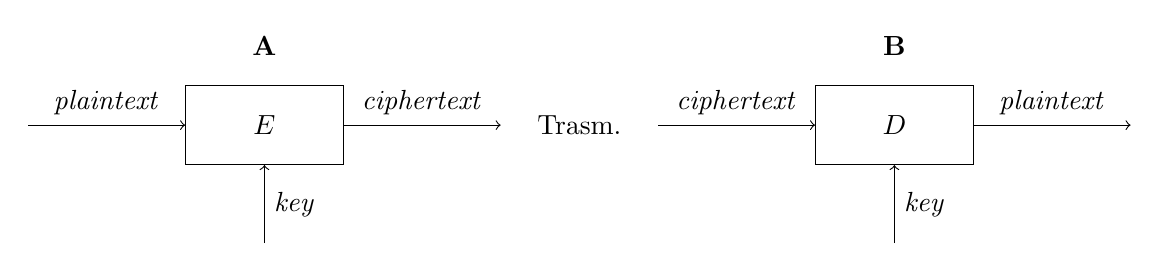
\begin{tikzpicture}
	\node at (4,0) [rectangle,draw, minimum width=2cm, minimum height=1cm] (E) {$E$};
	\draw (E);
	\draw[->] (1,0) -- (E) node[above, midway] {\textit{plaintext}};
	\draw[->] (4,-1.5) -- (E) node[right, midway] {\textit{key}};
	\draw[->] (E) -- (7,0) node[above, midway] {\textit{ciphertext}};
	\node at (8,0) (dots) {Trasm.};
	\node at (12,0) [rectangle,draw, minimum width=2cm, minimum height=1cm] (D) {$D$};
	\draw[->] (9,0) -- (D) node[above, midway] {\textit{ciphertext}};
	\draw[->] (12,-1.5) -- (D) node[right, midway] {\textit{key}};
	\draw[->] (D) -- (15,0) node[above, midway] {\textit{plaintext}};
	\node at (4,1) {\textbf{A}};
	\node at (12,1) {\textbf{B}};
	\end{tikzpicture}
	
	In crittografia si distinguono le due categorie \textit{a chiave simmetrica} e \textit{a chiave asimmetrica}. La differenza sta nel fatto che nella crittografia a chiave simmetrica le due entità che si scambiano il messaggio devono condividere una stessa chiave (che deve essere trasmessa su un canale sicuro), mentre nella crittografia a chiave asimmetrica le chiavi sono differenti e sono 2 per ogni entità, una pubblica e una privata. Nella crittografia a chiave asimmetrica si elimina il problema della condivisione della chiave; inoltre la chiave pubblica può essere compromessa da attaccanti senza che la chiave privata venga compromessa, e senza che venga compromessa la segretezza del messaggio.
	
	Un altro aspetto fondamentale della crittografia è che la cifratura e la decodifica sono facili, \textit{se le chiavi sono note}. Da ciò consegue che la sicurezza debba risiedere nella chiave, non nell'algoritmo in se.
	
	\subsection{Crittoanalisi}
	La scienza di recuperare il messaggio in chiaro senza conoscere il ciphertext si basa sostanzialmente su due differenti approcci:
	\begin{itemize}
		\item attacco brute-force;
		\item attacco crittoanalitico.
	\end{itemize}
	
	\paragraph{Attacco brute-force.} Un attacco bruteforce è semplice: consiste nel provare tutte le chavi possibili fino ad indovinare quella corretta. Questa tipologia di attacco in generale è sempre possibile nella sua semplicità, tuttavia, se la dimensione dello spazio delle chiavi inizia ad essere elevata, il tempo che si deve impiegare diventa insostenibile, per cui in questi casi è necessario ricorrere ad altri stratagemmi.
	
	\paragraph{Attacco crittoanalitico.} In questo caso si assume che l'attaccante conosca l'algoritmo utilizzato nella cifratura dei messaggi; si trova quindi una qualche debolezza nell'algoritmo che permetta di farlo fallire. 
	
	In tal senso, si tende a rendere noto un algoritmo affinchè il maggior numero di persone tenti di attaccarlo, per aumentare al massimo le possibilità che venga trovata una falla. (In contrasto con la cosiddetta \textbf{security by obscurity}).
	
	\paragraph{Tipologie di attacco.}Consideriamo ora i possibili attacchi che un sistema crittografico deve affrontare per essere affidabile:
	\begin{itemize}
		\item \textit{known cypertext attack:} questo attaccante è il meno aggressivo e conosce solamente il testo cifrato;
		
		\item \textit{known plaintext attack:} conosce entrambi i tipi di testo;
		
		\item \textit{choosen plaintext:} può scegliere il plaintext da codificare e analizzare il ciphertext ottenuto;
		
		\item \textit{adaptive choosen plaintext:} può liberamente scegliere il plaintext da far codificare e comportarsi di conseguenza, sulla base del risultato appena ottenuto.
		
		\item \textit{chosen ciphertext:} l'attaccante può scegliere differenti ciphertext e avere accesso al plaintext decriptato, per infine ricavare la chiave.
		\end{itemize}
	
	\subsection{Notazione} \label{notation}
	La notazione usata è la seguente: \begin{itemize}
		\item $\mathcal{A}$ è l'alfabeto, ovvero un insieme finito di simboli;
		\item $\mathcal{M} \subseteq \mathcal{A}^*\star$ è il messaggio, dove $M \in \mathcal{M}$ è il \textit{plaintext};
		\item $\mathcal{C}$ è il messaggio cifrato, il cui alfabeto può anche differire da quello usato per $M$;
		\item $\mathcal{K}$ indica lo spazio delle chiavi;
		\item ogni $e \in \mathcal{K}$ denota una funzione biiettiva da $\mathcal{M}$ a $\mathcal{C}$, viene indicata con $\encr$ ed è la funzione di cifratura;
		\item ogni $d \in \mathcal{K}$ è una funzione biiettiva da $\mathcal{C}$ a $\mathcal{M}$, indicata con $\decr$ ed è la funzione di decodifica.
	\end{itemize}

	Data la notazione soprastante, indichiamo con cifrario un insieme $\lbrace \encr\ |\ e \in \mathcal{K} \rbrace$ e il suo corrispondente $\lbrace \decr\ |\ d \in \mathcal{K} \rbrace$ tale che per ogni $e \in \mathcal{K}$ esiste un solo $d \in \mathcal{K}$, in modo tale che $\decr = \encr^{-1}$. La coppia $\langle e, d \rangle$ forma una coppia di chiavi, dove $e$ e $d$ possono anche essere identiche (come nel caso della crittografia simmetrica).
	
	\section{Crittografia a chiave simmetrica}
	Nella crittografia a chiave simmetrica le chiavi sono le stesse ($e = d$), e i due interlocutori condividono una chiave. I cifrari possibili nel caso della crittografia simmetrica sono di 3 categorie: \begin{itemize}
		\item \textit{cifrari a blocchi:} dividono il testo in blocchi di lunghezza fissa e cifrano un blocco alla volta;
		\item \textit{cifrari a flusso:} cifrari a blocchi in cui la dimensione di ogni blocco è fissata a 1;
		\item \textit{codes:} cifrari che lavorano su parole a lunghezza variabile.
	\end{itemize}

	\subsection{Tecniche di sostituzione}
	Sono tutti quei cifrari che sostituiscono una lettera con un'altra lettere, basandosi su una qualche regola di sostituzione, come il cifrario di Cesare e la permutazione casuale.
	
	\paragraph{Cifrario di Cesare.}
	Il messaggio viene cifrato sostituendo ogni lettera $l$ del messaggio con la $l+k$ esima lettera dell'alfabeto; la chiave quindi è data dalla coppia $(l, l+k)$. 
	
	Il cifrario di Cesare è facile da attaccare in quanto basta un attacco \textit{bruteforce}, quindi è sufficiente provare tutte le combinazioni (che sono in totale 26).
	
	\paragraph{Permutazione casuale.}
	Supponiamo di usare come cifrario una permutazione casuale dell'alfabeto, ovvero sostituendo ad ogni lettera dell'alfabeto un'altra lettera, in modo totalmente casuale. In tal caso l'attacco bruteforce richiederebbe tempo eccessivo (ci sono $26!$ pssibili combinazioni da provare, che sono decisamente troppe). 
	
	La tecnica usata per attaccare questo tipo di crittografia è l'\textit{analisi delle frequenze}, ovvero l'analisi delle lettere che capitano di più in una data lingua, e associare la lettera del messaggio cifrato con una data frequenza con quella nella lingua del messaggio con una frequenza simile.
	
	\paragraph{Cifrario di Vigenère.}
	Il cifrario di Vigenère riprende l'idea del cifrario di Cesare. L'idea è la seguente: presa una chiave (es. \textit{key}), si ripete la chiave tante volte quanto è lungo il testo (eventualmente troncando l'ultima ripetizione), e si codifica la lettera con il corrispondete cifrario di Cesare. \\
	
	\noindent
	K E Y K E Y K E Y K E Y \\
	P R O V A D I T E S T O \\
	
	
	La prima lettera del cipher text sarà la lettera ottenuta dal cifrario di Cesare di chiave $(K,P)$, la seconda con la chiave $(E, R)$ e così via.
	
	Anche questo cifrario è semplice da attaccare, si parte dalla divisione del ciphertext in gruppi di lunghezza pari a quella della chiave, e si esegue l'analisi delle frequenze su ogni gruppo.
	
	\subsection{Cifrari a trasposizione}
	Funzionano in maniera leggermente diversa. Dato un blocco di lunghezza $l$ e $\mathcal{K}$ un insieme di permutazioni su $\lbrace 1 \dots t \rbrace$, si ha che \[ \encr(m) = m_{e(1)}, \dots, m_{e(2)} \] Per decodificare si applica la permutazione inversa ad ogni carattere del ciphertext.
	
	\subsection{Cifrario di Feistel}
	
	\subsection{Data Encryption Standard (DES)}
	È un cifrario a blocchi che lavora su blocchi di 64 bit. Fu in effetti il primo standard di crittografia, e ne furono rilasciate versioni aggiornate che lavorassero su chiavi di lunghezza maggiore (3-DES). Non è ancora stato violato, ma è possibile ridurre in tempo lineare lo spazio delle chiavi da $2^{56}$ a $2^{43}$.
	
	\begin{center}
		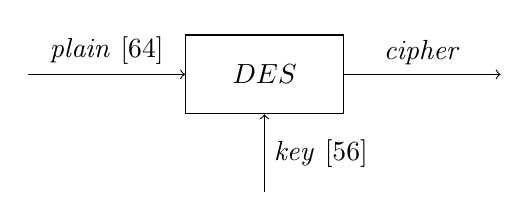
\begin{tikzpicture}
		\node at (4,0) [rectangle,draw, minimum width=2cm, minimum height=1cm] (E) {$DES$};
		\draw (E);
		\draw[->] (1,0) -- (E) node[above, midway] {\textit{plain} $\left[ 64 \right]$};
		\draw[->] (4,-1.5) -- (E) node[right, midway] {\textit{key} $\left[ 56 \right]$};
		\draw[->] (E) -- (7,0) node[above, midway] {\textit{cipher}};
		\end{tikzpicture}
	\end{center}
	
	\subsubsection{Double DES e 3-DES}
	La variante DD, che usa DES due volte consecutive, è soggetta ad un attacco del tipo \textit{Meet-in-the-Middle}.
	\begin{center}
		\begin{tikzpicture}
		\node at (4,0) [rectangle,draw, minimum width=2cm, minimum height=1cm] (E) {$DES$};
		\draw (E);
		\draw[->] (1,0) -- (E) node[above, midway] { $P_1$};
		\draw[->] (4,-1.5) -- (E) node[right, midway] {$K_1$};
		\draw[->] (E) -- (7,0) node[above, midway] {$M$};
		\node at (8,0) [rectangle,draw, minimum width=2cm, minimum height=1cm] (2E) {$DES$};
		\draw[->] (8,-1.5) -- (2E) node[right, midway] {$K_2$};
		\draw[->] (2E) -- (11,0) node[above, midway] { $P_2$};
		\end{tikzpicture}
	\end{center}

	L'attacco funziona nel seguente modo: \begin{enumerate}
		\item Dato un $C = E_{K_2}(E_{K_1}(P))$, sia $X = E_{K_1}(P) = D_{K_2}(C)$;
		\item Dati $P$ e $C$, cifrare $P$ per ogni possibile chiave (sono $2^{56}$);
		\item Generare una tabella con tutti i risultati, ordinati secondo $X$;
		\item Decifrare $C$ con tutte le possibili $K_2$, cercando un matching con quelle i risultati ottenuti prima. Ogni coppia è una possibile coppia valida, basta confrontare i risultati con $P$ e $C$ iniziali.
	\end{enumerate}

	In effetti, guardando lo schema sopra, si nota che al massimo occorrono $2^{56}$ operazioni per violare questo protocollo.
	
	Con 3-DES invece, un tentativo con la soluzione bruteforce necessita di almeno $2^{112}$ operazioni, un numero notevolmente più alto. Al momento infatti non esistono soluzioni per violare 3-DES.
	
	\subsection{Advanced Encryption Standard (AES)}
	Proposto come rimpiazzo di DES nel 1991, fu selezionato nel 2001. Infatti il DES iniziava a non andare più bene, in larga parte perchè era disegnato per i software degli anni 70 ed era abbastanza lento. AES funziona in maniera più snella e lavora su chiavi molto più lunghe (128, 192 e 256 bit).
	
	\subsection{Cipher block chaining}
	Come ci si comporta quando la lunghezza del messaggio eccede la dimensione del blocco? In tal caso, ci sono molteplici possibilità:\begin{enumerate}
		\item Splittare il messaggio in $m$ blocchi, e cifrarli individualmente. Questa opzione è soggetta a pesanti limtazioni, la prima data dal fatto che identici plaintext vengono mappati su identici ciphertext (\textit{information leak}); la seconda invece limita di parecchio le possibilità di individuare eventuali manomissioni del messaggio da parte di terzi (\textit{integrity});
		
		\item Si può pensare in alternativa di far dipendere un carattere del ciphertext da quello precedente: dato un valore iniziale, il successivo carattere sarà cifrato con uno XOR tra il carattere precedentemente cifrato e il carattere da cifrare. In sostanza, dato un certo $C_0$, \begin{align*}
			C_i &= E_K(P_i \oplus C_{i-1}) \\
			P_i &= C_{i-1} \oplus D_K(C_i) \quad \text{(per la decodifica)}
		\end{align*}
	\end{enumerate}

	Con la seconda soluzione, i caratteri cifrati dipendono strettamente da quelli precedenti, quindi è impossibile che due plaintext uguali vengano mappati su ciphertext uguali.
	
	\subsection{Posizionamento dei sistemi crittografici}
	Distinguiamo i casi di \textit{link encryption} e \textit{end-to-end encryption}.
	Nella link encryption ci sono sistemi di cifratura ad ogni collegamento, quindi i dati vengono decifrati e cifrati ad ognuno dei singoli collegamenti. Nella crittografia end-to-end invece, ciò che accade è che i sistemi di cifratura sono posizionati all'origine e alla destinazione dei dati, però in tal caso è necessario l'utilizzo di chiavi condivise tra i due interlocutori.
	
	Guardando la questione da un punto di vista alternativo, ossia quello dello stack OSI, possiamo osservare come la link encryption sia applicata ai livelli più bassi dello stack, mentre man mano si sale viene applicata una crittografia di tipo end-to-end. Idealmente, serve che la crittografia end-to-end protegga i dati contenuti nei pacchetti, ma che lasci inalterati gli header, per permettere l'inoltro dei pacchetti. La link encryption protegge invece i dati di inoltro da monitoraggio e analisi da parte di terzi.
	
	\subsection{Distribuzione delle chiavi}
	Come già detto in precedenza, la crittografia a chiave simmetrica richiede che le parti condividano una chiave. Ciò può costituire un problema, dal momento che terzi malintenzionati possono sempre tentare di rubare la chiave sfruttando qualche falla nel sistema di condivisione della stessa.
	
	Tipicamente non viene usata una sola chiave, ma una gerarchia di chiavi. Si ha quindi:\begin{itemize}
		\item \textit{session key:} usata per crittografare dati per una sola sessione logica;
		\item \textit{master key:} usata per cifrare le sessioni.
	\end{itemize}

	I problemi principali che si possono incontrare quindi sono i seguenti: \begin{itemize}
		\item la gerarchia delle chiavi è necessaria per reti molto vaste, ma è necessaria una sorta di garanzia sulle chiavi;
		
		\item il tempo di vita della chiave di sessione deve essere il minore possibile;
		
		\item l'uso di un sistema automatico di ditribuzione delle chiavi necessita la fiducia da parte degli utenti;
		
		\item il sistema di distribuzione è decentralizzato;
		
		\item è necessario stabilire una politica di controllo sull'uso delle chiavi.
	\end{itemize}

	\section{Crittografia a chiave pubblica}
	\paragraph{Notazione.} Oltre alla notazione specificata nella sezione \ref{notation}, specifichiamo con $PU_b$ e $PR_b$ rispettivamente la chiave pubblica di B e la chiave privata di B.
	
	\subsection{Struttura del sistema}
	Questo tipo di crittografia elimina il problema della distribuzione delle chiavi, in quanto ogni utente ha due chiavi, una pubblica (che tutti possono vedere), e una privata (che \textit{dovrebbe} rimanere incognita).
	
	Ogni utente genera una coppia di chiavi, una pubblica e una privata. Quella pubblica viene inserita in un registro.
	Supponiamo che B voglia inviare un messaggio ad A. La procedura è la seguente:\begin{enumerate}
		\item B cifra il messaggio con la chiave pubblica di A;
		\item A riceve il messaggio cifrato trasmesso da B;
		\item A decifra il messaggio ricevuto usando la sua chiave privata.
	\end{enumerate}

	\subsection{Crittoanalisi della crittografia a chiave pubblica}
	Gli attacchi possibili sono i seguenti: \begin{itemize}
		\item \textit{Bruteforce:} l'unica soluzione è aumentare la lunghezza della chiave, cosa che potrebbe non scalare bene con l'aumentare della dimensione, data la complessità dell'algoritmo; in pratica la crittografia a chiave pubblica viene usata solamente per la gestione delle chiavi e la firma digitale;
		
		\item \textit{Calcolo di} $PR_b$ \textit{data} $PU_b$: di questo attacco non esiste prova nè controprova;
		
		\item \textit{Probable-message attack:} supponiamo di avere un messaggio $M$ abbastanza corto, tale che sia $C = E(\pua, M) $, l'attaccante potrebbe calcolare tutti i $Y_i = E(\pua, M)$ per tutti i possibili plaintext, e fermarsi quando $Y_i = C$. La  soluzione a questo tipo di attacco è banale, basta appendere alcuni bit random alla fine di $M$, in modo tale da impedire di trovare un $Y_i$ valido.
	\end{itemize}

	Il vantaggio è evidente: senza doversi scambiare le chiavi, A è certa che il messaggio non sia stato letto in precedenza, in quanto è decifrabile solo con la chiave privata che solo lei possiede. Le applicazioni sono molteplici: si va dalla firma digitale, alla cifratura/decifratura di contentuti, fino allo scambio di chiavi.
	
	\subsection{Requisiti necessari per il funzionamento}
	Come per la crittografia a chiave simmetrica, ci sono dei requisiti fondamentali al sistema per garantire un processo di crittografia che sia ottimale: \begin{itemize}
		\item deve essere facile generare la coppia di chiavi;
		\item deve essere facile, per il mittente A, generare $C=E(PU_b, M)$;
		\item deve essere facile, per il destinatario B, calcolare $M=D(PR_b, C)$;
		\item deve essere difficile, per un attaccante, ottenere la chiave privata da quella pubblica;
		\item deve essere difficile, per un attaccante, data la chiave pubblica e il ciphertext, ottenere il messaggio in chiaro.
	\end{itemize}

	\subsection{Algoritmo RSA}
	\begin{definit}[One-way function]
		Definiamo one-way function una funzione $f:X \to Y$ dove $f$ è facile da calcolare $\forall x \in X$, ma è molto difficile da calcolare la sua inversa $f^{-1}$.
	\end{definit}

	\begin{definit}[Trapdoor one-way function]
		Una trapdoor one-way function è una funzione $f_k:X \to Y$ dove, data un'informazione extra $k$ (trapdoor) è calcolabile, $\forall y \in Im(f)$, una $x\in X \text{ t.c. } f_k(x)=y$.
	\end{definit}

	L'algoritmo RSA è usato in molti degli standard odierni, ma ha lo svantaggio di essere circa 1000 volte più lento di DES, oltre ad avere bisogno di chiavi abbastanza lunghe (1024 bit è relativamente sicura) ed essere vulnerabile ad alcuni tipi di attacco.
	
	La cifratura e la decifratura iniziano da un numero noto sia ad A che a B. Il plaintext viene quindi splittato in blocchi di lunghezza pari a $\lceil log_2(n) \rceil$, in modo tale che ogni blocco rappresenti un numero $M$ per cui $M < n$. Il ciphertext è definito come \[ C=M^e \mod n \] mentre il plaintext è ricavabile tramite \[ M = C^d \mod n = M^{ed} \mod n \]
	
	Le chiavi privata e pubblica sono date rispettivamente da $\lbrace d,n \rbrace$ e $\lbrace e,n \rbrace$. Perchè l'algoritmo funzioni, devono essere soddisfatti i seguenti vincoli:\begin{itemize}
		\item $\exists e,d,n. M^{ed} \mod n = M, \forall M<n$;
		\item è facile calcolare $M^e \mod n$ e $C^d \mod n$;
		\item è impossibile determinare $d$ conoscendo $e$ ed $n$.
	\end{itemize}
	
	Per generare una coppia di chiavi si usano i seguenti passi: \begin{enumerate}
		\item Si generano due numeri primi $p$ e $q$ (possibilmente grandi);
		\item Si calcolano $n=p*q$ e $\phi = (p-1)(q-1)$;
		\item Si seleziona un $e$, $1 < e < \phi$;
		\item Si determina $d = e^{-1} \mod \phi$;
		\item Si pubblica la chiave $(e,n)$ e si mantiene privata $(d,n)$. 
	\end{enumerate}

	La sicurezza di RSA risiede nel fatto che ricavare $d$ data la chiave pubblica è estremamente complesso, dal momento che sarebbe necessario trovare $d = e^{-1} \mod \phi$; non si conoscono algoritmi polinomiali per fare ciò.
	
	\subsection{Distribuzione delle chiavi}
	Il problema risiede nella fiducia da riporre in un sistema di distribuzione delle chiavi dove le chiavi stesse non possano venire compromesse. Si usano in tal senso gli algoritmi crittografici a chiave asimmetrica. 
	
	\subsubsection{Distribuzione con RSA}
	Lo scambio delle chiavi con RSA è abbastanza semplice: dato un $m$ e scelta una chiave $k$ casuale, si cifra un \[ c=(k^e \mod n, E_k(m)) \]
	
	La decifratura delle chiavi, con la chiave privata $(d,n)$, avviene splittando il ciphertext in due blocchi separati, con \begin{align*}
		k &= c^d_1 \mod n \\
		m &= D_k(c_2)
	\end{align*}
	
	L'unico problema è che se la chiave privata è compromessa, allora $k$ può essere recuperata da un intruso dal traffico precedentemente intercettato.
	
	\subsubsection{Diffie-Hellman}
	\begin{definit}[Primitive root]
		Una primitive root $s$ di un numero primo $p$ è il numero le cui potenze generano $1,\dots,p-1$.
	\end{definit}

	\begin{definit}[Logaritmo discreto]
		Definiamo il logaritmo discreto di $b$ come un valore $i$ tale che $b=s^i \mod p$.
	\end{definit}
	
	Il calcolo del logaritmo discreto sembra essere infattibile, quindi è possibile strutturare un sistema crittgrafico che sfrutti questa caratteristica.
	
	\paragraph{Generazione delle chiavi.} La generazione delle chiavi segue le seguenti fasi: \begin{enumerate}
		\item I due enti si scambiano un numero primo $q$ e una primitive root $\alpha$, entrambe pubbliche;
		\item A e B generano due numeri $X_A$ e $X_B$, entrambi minori di $q$;
		\item A calcola $Y_A = \alpha^{X_A} \mod q$ (analogamente B calcola $Y_B$);
		\item A e B si scambiano i risultati;
		\item A calcola $K_A = Y_B^{X_A} \mod q$, B fa l'analogo con $X_B$. Le due chiavi risultano essere uguali ora.
	\end{enumerate}

	\paragraph{Punti di forza.} Notare quali sono i punti di forza di Diffie-Hellman: la chiave è creata senza avere alcuna informazione iniziale e non è mai trasmessa (viene trasmesso solo $Y$)
	
	Diffie-Hellman gode inoltre della proprietà di \textit{perfect forward secrecy}, ossia la garanzia che le chiavi di sessione non potranno mai essere compromesse se una delle chiavi a lungo termine viene compromessa.
	
	\paragraph{Debolezze.} Le chiavi generate non sono autenticate, quindi sono vulnerabili ad un attacco del tipo MITM.
	Supponiamo infatti che nella trasmissione vengano intercettate $Y_A$ e $Y_B$: in tal caso $Z$ può calcolare le due chiavi che sarebbero calcolate da $A$ e $B$, mentre $A$ e $B$ calcolano le relative chiavi ma utilizzando $Y_Z$ al posto dei rispettivi $Y$.
	
	Una possibile soluzione a tale problema potrebbe essere la firma digitale, ma ciò richiede l'utilizzo di una chiave condivisa.
	
	\subsection{Integrità dei messaggi}
	L'integrità è la proprietà che garantisce che i messaggi non sono in alcun modo stati alterati da una fonte non autorizzata. Questa proprietà viene garantita tramite funzioni di hash, ovvero funzioni che soddisfano le seguenti proprietà: \begin{itemize}
		\item \textit{Compressione:} dato $x$ come input, $h(x) $ ritorna sempre un output di lunghezza fissa;
		\item Sono calcolabili in tempo polinomiale.
	\end{itemize}
	
	La funzione $h(x)$ è una \textit{funzione hash crittografica} se:\begin{itemize}
		\item è \textit{one-way}, ossia dato $y$ è difficile calcolare $x \text{ t.c. } h(x) = y$;
		\item è difficile trovare un secondo input $x'$ tale che $h(x) = h(x')$ (\textit{collision resistance, 2nd preimage resistance})
	\end{itemize}
	
	\paragraph{Birthday attack.} Un \textit{birthday attack} sfrutta il paradosso del complanno. Supponiamo che A e B vogliano siglare un contratto, ma B vuole ingannare A facendogliene firmare uno fraudolento. B genera tanti contratti $x$ corretti, modificandoli in modo da non cambiarne il significato, e fa altrettanto con i contratti fraudolenti $y$. A questo punto basta trovare due contratti $x_i$ e $y_i$ tali che $h(x_i) = h(y_i)$. B a questo punto fa firmare ad A $x_i$, ma, dato che gli hash sono uguali, può usare la firma per rendere vero anche il contratto fraudolento $y_i$.
	
	\subsubsection{Costruzione di una funzione hash crittografica}
	Uno dei metodi più semplici consiste nell'usare una tecnica di block-chaining.
	Si divide il messaggio in $m$ blocchi, e si usa un algoritmo simmetrico per cifrarli uno per volta, cifrando il blocco $m_i$ usando $E(m_{i-1})$. Tuttavia gli algoritmi moderni usano tecniche più complesse, alcuni dei quali sono:\begin{itemize}
		\item MD5 (hash di 128 bit, con debolezze note);
		\item SHA (hash di 160 bit, considerato sicuro).
	\end{itemize}

	\subsection{Autenticazione dei messaggi}
	L'autenticazione dei messaggi (che implica l'integrità) garantisce la fonte del messaggio. I metodi usati per garantirla sono i MAC e le firme digitali.
	
	\subsubsection{Message Authentication Code}
	Un algoritmo MAC è dato da una famiglia di funzioni hash $h_k$ (parametrizzate dalla chiave $k$), che devono essere \textit{computation-resistant}, ossia, data una o più coppie $(x_i, h(x_i))$, deve essere difficile calcolare $(x, h(x))$ dato un qualsiasi $x \neq x_i$.
	
	L'autenticità con il MAC è verificata controllando dal lato del destinatario che, se $MAC = h_k(M)$, valga $MAC' = h_k(M')$
	
	La costruzione di un MAC avviene usando il cipher-block chaining. Dati $n$ blocchi, si calcola \begin{align*}
		c_1 &= E_K(m_1 \oplus 0) \\
		c_i &= E_K(c_{i-1} \oplus m_i)
	\end{align*}
	
	Alla fine, il blocco $c_n$ sarà il MAC totale.
	
	\subsubsection{Firme digitali}
	Lo scopo della firma digitale è dimostrare che un messaggio è stato mandato da una specifica persona, ed è fondamentale per i concetti di autenticazione e non-ripudio. Dati: \begin{itemize}
		\item $\mathcal{M}$ l'insieme dei messaggi firmabili;
		\item $\mathcal{S}$ l'insieme delle firme (stringhe di $n$ bit);
		\item $S_A:\mathcal{M} \to \mathcal{S}$ è la trasformazione di firma per A (deve rimanere segreta);
		\item $V_A:\mathcal{M} \times \mathcal{S} \to \left\{true, false \right\}$ è la trasformazione di verifica per A, ed è pubblica.
	\end{itemize}

	Lo schema di firma è quindi dato da $S_A$ e $V_A$.
	\paragraph{Procedura di firma e verifica.} La procedura di firma è semplice: dato $m \in \mathcal{M}$, A calcola $s=S_A(m)$ e trasmette $(m,s)$. La procedura di verifica per A consiste nel calcolare $u=V(m,s)$. Se $u=true$ allora la firma è verificata.
	
	\paragraph{Implementazione del meccanismo di firma.}
	Lo schema per un possibile protocollo di firma reversibile (che usa crittografia simmetrica) funziona nel modo seguente: \begin{itemize}
		\item siano $M$ e $C$ il messaggio e la signature;
		\item siano $e,d$ le chiavi usate per cifrare/decifrare;
		\item definiamo come funzione di firma $S_A = D_d$;
		\item definiamo quindi la verifica $V_A = \begin{cases}
			true &\text{if } E_e(s) = m; \\
			false &\text{otherwise}
		\end{cases}$
	\end{itemize}

	Questo schema è passibile di \textit{forgery attack}:\begin{enumerate}
		\item un attaccante B seleziona una $s \in S$ random e calcola $m = E_e(s)$;
		\item dato che $M=S$, può submittare $(m,s)$ come messaggio con signature;
		\item la verifica ritorna \textit{true} anche se A non ha firmato $M$.
	\end{enumerate}
	
	La soluzione è identificare come $\mathcal{M}'$ un sottoinsieme dei messaggi firmabili, e ridefinire $V_A$ in modo che dia true solo se $E_e(s) \in \mathcal{M}'$. In tal modo il messaggio può essere recuperato, e si ottiene un protocollo tanto sicuro quanto più piccolo è $\mathcal{M}'$ .

	RSA costituisce un meccanismo di firma, dal momento che la forgery è prevenuta firmando i messaggi con una struttura fissa, ossia un hash firmato, mandato col messaggio.
a
	\section{Public Key Infrastructures}
	Una PKI è una infrastruttura che consente agli utenti di correlare una chiave ad un altro utente.
	Per registrare una chiave presso una CA (\textit{Certification Authority}), un utente deve prima generare la sua coppia di chiavi e consegnare la chiave pubblica alla CA, la quale poi firma un certificato digitale che associa l'utente alla chiave.

	Oltre al mantenimento delle chiavi, la PKI fornisce il servizio di revoca, recovery e aggiornamento delle chiavi.

	I componenti di una PKI (sia aperta che chiusa) sono i seguenti: \begin{itemize}
			\item \textbf{Certification Authority:} crea e mantiene le directory e la CRL (Certificate Revocation List);
			\item \textbf{Directory:} rende disponibili la CRL e i certificati e deve identificare in modo univoco gli utenti;
			\item \textbf{Registration Authority:} sovrintende il processo di registrazione degli utenti e ne gestisce l'autenticazione.
	\end{itemize}

    \subsection{Certificati}
    Un certificato è semplicemente un token che collega una chiave ad un'identità. Per costruire un certificato la CA firma con la sua chiave privata un messaggio contenente la rappresentazione dell'utente titolare della chiave e la sua chiave pubblica, insieme ad un timestamp.

    Il problema tuttavia si ripercuote sulla CA. Come si può validare il certificato della CA? Ci sono due possibili approcci: \begin{itemize}
        \item costruire una gerarchia ad albero con la root trustata a priori;
        \item arrangiare una fiducia collettiva tra tutti.
    \end{itemize}

    \paragraph{Certificati X.509.} Sono un tipo di certificato standard ora utilizzato da moltissime applicazioni (IPSEC, SSL/TLS, ecc.), e sono basati sull'uso di crittografia a chiave pubblica (RSA raccomandato).

    Un normale certificato X.509 è composto dai seguenti campi: \begin{itemize}
        \item \textbf{Serial number:} unico tra i certificati;
        \item \textbf{Signature alg. identifier:} identificatore dell'algoritmo usato per firmare il certificato;
        \item \textbf{Issuer name:} la CA che ha firmato il certificato;
        \item \textbf{Periodo di validità};
        \item \textbf{Subject name:} nome dell'utente a cui il certificato si riferisce (l'utente la cui chiave è certificata);
        \item \textbf{Subject PK info:} informazioni sulla chiave pubblica dell'utente;
        \item \textbf{Signature:} l'hash di tutti gli altri campi, firmato con la chiave pubblica della CA.
    \end{itemize}

    Se un utente vuole accedere ad un certificato e verificare la chiave di un utente procede come segue:
    \begin{enumerate}
        \item L'utente decifra la signature con la chiave pubblica della CA;
        \item Usa le informazioni della signature per calcolare l'hash degli altri campi, che confronta con quello contenuto nella signature (se corrispodono il certificato è valido);
        \item Controlla il periodo di validità per verificare che la chiave sia ancora valida.
    \end{enumerate}

    \paragraph{Modelli fiduciari.}
    Per stabilire la validità di un certificato esistono vari modelli di fiducia che stabiliscono in che modo gli utenti si fidano delle CA.

    \begin{itemize}
        \item \textbf{Fiducia diretta.} Ogni utente iscritto ad una CA si fida di tutti gli altri iscritti a quella CA. Tutti i certificati sono nella stessa directory.
        
        \item \textbf{Fiducia gerarchica.} Per molti utenti è più comodo avere molte CA, ognuna coprente una porzione degli utenti totali. Le CA vengono ordinate in maniera gerarchica ad albero, in cui ogni nodo non-foglia è certificato dai nodi soprastanti.

        \textbf{Cross certification:} se le CA si sono scambiate le corrispondenti chiavi pubbliche, allora due utenti registrati presso due CA diverse possono ottenere le rispettive chiavi attraverso una \textbf{catena di certificati}.
    \end{itemize}

    
    \paragraph{Key revocation.}
    Come specificato in precedenza, la CA mantiene una CRL. Un certificato può essere revocato per svariate motivazioni: \begin{itemize}
        \item la chiave privata dell'utente è stata compromessa;
        \item l'utente non è più registrato presso quella CA;
        \item il certificato della CA è compromesso.
    \end{itemize}

    \section{Realizzazione e verifica di protocolli}
    Prima di passare a come si realizza un protocollo, diamo alcune fondamentali definizioni.
    \begin{definit}
        Un protocollo consiste in un insieme di regole che determinano come avviene lo scambio di messaggi tra due utenti.
    \end{definit}

	Un protocollo di sicurezza usa meccanismi di tipo crittografico per raggiungere determinati obiettivi di sicurezza.
	
	Per la costruzione di un protocollo è necessario stabilire una notazione di tutti gli elementi coinvolti:
	\begin{itemize}
		\item Entità che partecipano;
		\item Le chiavi necessarie sono:
			\begin{itemize}
				\item cifratura: $\lbrace M\rbrace_K$ ($\lbrace M\rbrace_{K_A}$ è la cifratura con la chiave pubblica di A);
				\item firma: $\lbrace M\rbrace_{K^{-1}}$ (la firma con la chiave privata di A è $\lbrace M\rbrace_{K_A^{-1}}$)
				\item nel caso di chiavi simmetriche si usa $\lbrace M\rbrace_{K_{AB}}$
			\end{itemize}
		\item Nonces: $NA, N1, \dots$ numeri usati per le fasi di challenge/response;
		\item Timestamps $T$, usati per la validità delle chiavi.
	\end{itemize}

	Una singola comunicazione tra due entità è indicata come \[ A \to B : \lbrace A, T_1, K_{AB}\rbrace_{K_B} \]

	È inoltre necessario fare delle assuzione sulle capacità dell'attaccante:
	\begin{enumerate}
		\item Eavesdropping completo su tutti i messaggi mandati;
		\item Modifica e re-routing di tutti i messaggi;
		\item L'avversario può essere uno dei principals, oppure esterno, oppure anche una combinazione dei due;
		\item L'avversario è capace di ottenere il valore di tutte le precedenti chiavi di sessione (replay attack).
	\end{enumerate}

	\subsection{Protocollo di Needham - Schroeder (NSPK)}
	È un protocollo di scambio di chiavi, procede come segue:
	\begin{enumerate}
		\item $A \to B: \lbrace NA, A\rbrace_{K_B}$;
		\item $B \to A: \lbrace NA, NB\rbrace_{K_A}$;
		\item $A \to B: \lbrace NB\rbrace_{K_B}$
	\end{enumerate}

	Il protocollo opera assumendo che i principals possano generare nonces, e conoscano ognuno la chiave pubblica dell'altro.

	Gli obiettivi del protocollo sono:
	\begin{itemize}
		\item Autenticità dei messaggi;
		\item Garantire la timeliness dei messaggi (no replay attack);
		\item Garantire la sicurezza di specifici assets (ovvero le chiavi generate).
	\end{itemize}

	Il protocollo NSPK fu provato essere vulnerabile ad un attacco di tipo MITM. Fu migliorato semplicemente agguingendo alla risposta di B il nome di B. In tal modo A riceve il nome di B, si rende conto di aver scambiato il precedente messaggio con un intruso e chiude il canale.
	
	\subsection{Esempi di protocolli vulnerabili}
	Definiamo prima un elenco delle tipologie di attacco disponibili ad un attaccante del tipo assunto alla sezione precedente:
	\begin{itemize}
		\item Man-in-the-middle (parallel sessions): $A \leftrightarrow Z \leftrightarrow B$;
		\item Replay attack: riusa parti di messaggi precedenti;
		\item Masquerading attack: Z convince altri principals che la chiave di A sia $K_Z$
		\item Reflection attack: manda l'informazione trasmessa di ritorno al mittente;
		\item Oracle attack: sfrutta la disponibilità di un sistema a poter essere usato come oracolo (si/no);
		\item Type flaw attack: sostituisce il campo di un messaggio con un contenuto diverso (il nome per la chiave ad esempio).
	\end{itemize}
	
	L'esempio più classico è l'attacco MITM sul protocollo di Diffie-Hellman, a meno che non usi chiavi autenticate.

	\paragraph{Type-flaw attack.} Ci sono vari esempi di type-flaw attacks.
	Gli esempi più classici sono il protocollo Otway Rees (Authenticated server based key distribution), e l'Andrew Secure RPC.

	Nel caso Otway-Rees, il protocollo è così composto: \begin{align*}
		M_1. A \to B&: I,A,B, \lbrace N_A, I, A, B\rbrace_{K_{AS}} \\
		M_2. B \to S&: I,A,B, \lbrace N_A, I, A, B\rbrace_{K_{AS}}, \lbrace N_B, I, A, B\rbrace_{K_{BS}} \\
		M_3. S \to B&: I, \lbrace N_A, K_{AB}\rbrace_{K_{AS}}, \lbrace N_B, K_{AB}\rbrace_{K_{BS}}\\
		M_4. B \to A&: I, \lbrace N_A, K_{AB}\rbrace_{K_{AS}}
	\end{align*}

	Le chiavi del server sono note e I indica una run del protocollo.
	La vulnerabilità risiede nel fatto che, supponendo $\vert \lbrace I,A,B\rbrace\vert = \vert\lbrace K_{AB} \rbrace\vert$, un attaccante può inoltrare un messaggio del tipo 1 come messaggio del tipo 4. In tal modo $A$ vede il suo nonce e accetta $(I, A, B)$ come chiave di sessione.

	Per questo protocollo si prostpetta un secondo scenario di attacco, ovvero quello in cui l'attaccante fa da server, e inoltre a B, invece della chiave, la tripla $(I, A, B)$. In tal modo B e A usano $(I, A, B)$ come chiave e la secrecy non vale più.
	
	Nel caso Andrew-Secure RPC, il protocollo funziona così: \begin{align*}
		M_1. A \to B&: A, \lbrace N_A\rbrace_{K_{AB}}\\
		M_2. B \to A&: \lbrace N_A +1, N_B\rbrace_{K_{AB}}\\
		M_3. A \to B&: \lbrace N_B + 1\rbrace_{K_{AB}}\\
		M_4. B \to A&: \lbrace K'_{AB}, N_B'\rbrace_{K_{AB}}\\
	\end{align*}

	$K'_{AB}$ è la chiave di sessione e $N'_B$ è il nonce per la sessione seguente. L'attaccante può muoversi in modo che, in $M_4$, la chiave scambiata sia $N_A + 1$, previa intercettazione di $M_2$. Ciò nonostance, la segretezza dei messaggi non è violata.

	\paragraph{Protocollo Denning - Sacco.}
	Il protocollo si svolge in 3 passi: \begin{align*}
		A\to S&: A, B \\
		S\to A&: C_A, C_B \\
		A \to B&: C_A, C_B, \lbrace\lbrace T_A, K_{AB}\rbrace_{K_A^{-1}}\rbrace_{K_B}
	\end{align*}

	dove: \begin{itemize}
		\item $S$ è un server che funge da CA;
		\item $K_{AB}$ chiave di sessione segreta;
		\item $K_B$ chiave pubblica di B;
		\item $K_A^{-1}$ chiave privata di A, usata per firma;
		\item $C_A, C_B$ sono i certificati per A e B;
		\item $T_A$ timestamp generato da A.
	\end{itemize}

	Il punto di forza di questo protocollo risiede nel fatto che B è sicuro che la chiave pubblica sia di A in quanto è firmata con la sua chiave privata, il tutto cifrato con la chiave pubblica di B, il che indica che il messaggio è per B. Come extra, la chiave di A è provata da $C_A$.

	Questo protocollo è vulnerabile ad un MITM, ma è risolvibile aggiungendo i nomi di A e B insieme al timestamp e la chiave. In tal modo è facile verificare se qualcuno usa la propria chiave per modificare la cifratura della firma.

	\paragraph{Parallel sessions attack.} Consideriamo un semplice (ed estramamente lazy) protocollo di autenticazione: \begin{align*}
		M_1. A \to B&: \lbrace N_A\rbrace_{K_{AB}}\\
		M_2. B \to A&: \lbrace N_A + 1 \rbrace_{K_{AB}}
	\end{align*}
	Il protocollo è vulnerabile ad un attacco di tipo parallel sessions (con oracolo).
	L'attacco è banale:

	\begin{align*}
		M_1. A \to I&: \lbrace N_A\rbrace_{K_{AB}}\\
		M_2. I \to A&: \lbrace N_A \rbrace_{K_{AB}}\\
		M_3. A \to I&: \lbrace N_A + 1\rbrace_{K_{AB}}\\
		M_4. I \to A&: \lbrace N_A + 1 \rbrace_{K_{AB}}
	\end{align*}

	L'unica soluzione a questo attacco è, come nei casi precedenti, aggiungere il nome di A nel messaggio cifrato.

	\paragraph{Replay attack.} Consideriamo il protocollo Needham-Schroeder per chiavi condivise: \begin{align*}
		M_1. A \to S&: A, B, N_1 \\
		M_2. S \to A&: \lbrace N_1, B, K_{AB}, \lbrace K_{AB}, A\rbrace_{K_{BS}} \rbrace_{K_{AS}} \\
		M_3. A \to B&: \lbrace K_{AB}, A\rbrace_{K_{BS}} \\
		M_4. B \to A&: \lbrace N_2\rbrace_{K_{AB}}\\
		M_5. A \to B&: \lbrace N_2-1\rbrace_{K_{AB}}
	\end{align*}

	Tale protocollo è passabile di replay attack, in quanto un qualsiasi attaccante Z, supponendo che abbia recuperato la chiave di una precedente run del protocollo ($K'_{AB}$), potrebbe agire come segue:
	\begin{align*}
		M_3. Z \to B&: \lbrace K'_{AB}, A\rbrace_{K_{BS}} \\
		M_4. B \to A&: \lbrace N_2\rbrace_{K'_{AB}}\\
		M_5. A \to B&: \lbrace N_2-1\rbrace_{K'_{AB}}
	\end{align*}
	
	In tal modo verrebbe compromessa la segretezza dei messaggi. Un possibile fix è quello di aggiungere dei timestamp da usare come timeout, oppure aggiungere un handshake extra all'inizio del protocollo.
	
	\section{Kerberos}
	Kerberos è un protocollo di autenticazione in ambienti distribuiti. È costruito su alcuni principi di base: \begin{itemize}
		\item Sicurezza (no eavesdropping);
		\item Affidabilità;
		\item Trasparenza: l'utente usa un password singola per l'accesso alla rete, ignaro dei protocolli sottostanti (SSO);
		\item Scalabilità: il sistema deve essere in grado di supportare molti utenti/servizi alla volta.
	\end{itemize}
	
	\subsection{Architettura e funzionamento}
	L'architettura Kerberos è strutturata come segue: \begin{itemize}
		\item KAS (\textit{Kerberos Authentication Server}) per l'autenticazione;
		\item TGS (\textit{Ticket Granting Server}) per l'autorizzazione;
		\item Servizi di controllo dei ticket.
	\end{itemize}
	
	Supponiamo ora che un utente voglia accedere ad un servizio. L'architettura funziona come segue: \begin{enumerate}
		\item L'utente richiede il servizio, richiedendo al KAS un ticket-granting ticket;
		\item Il KAS verifica l'accesso, genera il ticket e crea la chiave di sessione. Il tutto viene cifrato con una chiave calcolata usando la psw di accesso.
		\item La workstation dell'utente chiede la password, che usa per decifrare il messaggio in arrivo, poi manda l'authenticator (username, indirizzo di rete e timestamp attuale) al TGS;
		\item il TGS decifra il tutto, verifica la richiesta, genera il ticket per il server con il servizio richiesto e manda il tutto alla workstation;
		\item La workstation manda il ticket per il server e l'authenticator al server stesso;
		\item Il server verifica che ticket e authenticator matchino, quindi da accesso al servizio. Se è richiesta autenticazione mutuale, il server manda indietro il suo authenticator.
	\end{enumerate}

	È importante sottolineare che la fase 1 e 2 (\textbf{autenticazione}) sono svolte ad ogni sessione di login, i messaggi 3 e 4 (\textbf{autorizzazione}) sono svolti per ogni tipo di servizio mentre i messaggi 5 e 6 (\textbf{accesso al servizio}) sono scambiati ad ogni accesso al servizio.

	\paragraph{Autenticazione.} La fase di autenticazione procede come: \begin{align*}
		1.A \to KAS&: A, TGS \\
		2.KAS \to A&: \lbrace K_{A, TGS}, TGS, \mathcal{T}_1, \lbrace A, TGS, K_{A, TGS}, \mathcal{T}_1  \rbrace_{K_{KAS, TGS}}\rbrace_{K_AS}
	\end{align*}

	La sezione $\lbrace A, TGS, K_{A, TGS}, \mathcal{T}_1  \rbrace_{K_{KAS, TGS}}$ è l'\textit{AuthTicket}. $K_{A, TGS}$ ha un lifetime di alcune ore. 

	\paragraph{Autorizzazione.}
	La fase di autorizzazione contiene i messaggi 3 e 4, ovvero \begin{align*}
		3.A \to TGS&: \text{\textit{AuthTicket}}, \lbrace A, T_2\rbrace_{K_{A, TGS}}, B\\
		4.TGS \to A&:\lbrace K_{AB}, B, T_3, \lbrace A, B, K_{AB}, T_3\rbrace_{K_{B, TGS}} \rbrace_{K_A, TGS}
	\end{align*}

	La sezione del messaggio 3 $\lbrace A, T_2\rbrace_{K_{A, TGS}}$ è l'\textit{autenticator}, che ha un periodo di validità molto ridotto (secondi). Lo scopo dell'autenticator è quello di scongiurare eventuali replay attacks. Il TGS fornisce la chiave $K_{AB}$ con lifetime di alcuni minuti, e un \textit{ServTicket} ($\lbrace A, B, K_{AB}, T_3\rbrace_{K_{B, TGS}}$)

	\paragraph{Service phase.} La fase di accesso al servizio procede con i messaggi 5 e 6, ovvero: \begin{align*}
		5. A \to B&: \text{\textit{ServTicket, Authenticator}}\\
		6. B \to A&: \lbrace T_4 + 1\rbrace_{K_{AB}}
	\end{align*}

	Dopo la risposta del server, l'utente è autenticato e può iniziare ad usare il servizio.

	\subsection{Scalabilità}
	Definiamo \textit{realm} lo spazio definito da un server Kerberos. Il server salva username e password solo per gli utenti del suo realm. Tuttavia, una grande rete potrebbe essere divisa in più realms. Per questo motivo Kerberos è dotato anche di protocolli inter-realm, dove i server si registrano l'un l'altro e, nel caso un utente dovesse accedere ad un servizio posizionato in un altro realm, il KAS fornisce il ticket per accedere al TGS dell'altro realm. \\

	Kerberos 4 è soggetto a particolari limitazioni, quali il possibile flooding del KAS da parte di un attaccante, e la pesantezza della doppia crittografia, rimossa in Kerberos 5.

	Tutto il meccanismo inotre si basa sulla sincronizzazione dei timestamp, pertanto, se un host dovesse essere compromesso, per l'attaccante potrebbe essere possibile modificare i timestamps e attuare un replay attack.

	\section{SSL/TLS}
	TLS è un protocollo nato dall'evoluzione di SSL, che garantisce una cifratura end-to-end anche in presenza di una rete compromessa. TLS è composto da un \textbf{Record Protocol} che protegge i dati scambiati tra client e server, e l'\textbf{Handshake protocol}, reponsabile della fase di handshake tra le parti.

	\subsection{SSL Handshake}
	L'handshake è composto di 4 fasi: \begin{enumerate}
		\item Decisione dei protocolli crittografici da adottare;
		\item Scambio di chiavi del server;
		\item Scambio di chiavi del client;
		\item Fine, connessione online.
	\end{enumerate}

	\paragraph{Decisione dei protocolli.} I messaggi scambiati in questa fase sono 2: \begin{enumerate}
		\item \lstinline{client_hello}: il client invia al server un messaggio $\lbrace A, N_A, S_{id}, P_A\rbrace$, contenente il nome di A, un nonce, il session id e le preferenze sugli algoritmi per lo scambio delle chiavi e di compressione;
		\item \lstinline{server_hello:} lo stesso messaggio, ma con gli algoritmi e il nonce del server.
	\end{enumerate}

	\paragraph{Scambio chiave del server.} Il sever manda al client un certificato X.509v3 (\lstinline{server_certificate}) $cert(S, K_S)$. Notare che in realtà il protocollo prevede che si possa anche negoziare l'algoritmo per lo scambio delle chiavi e anche richiedere un certificato per il client (supponendo che il client abbia un propria chiave pubblica).

	\paragraph{Scambio chiavi del client.} Il client risponde con: \begin{enumerate}
		\item \lstinline{client_certificate}: il proprio certificato (se può);
		\item \lstinline{client_key_exchange}: \textit{pre-master secret}, PMS, cifrato con la chiave pubblica del server (arrivata tramite il certificato della fase 2). Il PMS sarà usato per calcolare il \textit{master secret} $M$, che ha utilizzi più avanti;
		\item \lstinline{certificate_verify}: la risposta al controllo di validità del certificato. 
	\end{enumerate}

	\paragraph{Fine della comunicazione.} Client e server si scambiano due messaggi \lstinline{finish}, cifrati con chiavi simmetriche generate dai nonce e $M$. Il messaggio di finish è un hash dei precedenti messaggi, garantendo integrità di tutti i messaggi precedenti.

	\subsection{Attacchi ad SSL}
	\paragraph{Version rollbcack attack.} L'attaccante trickava il server ad usare un versione più vecchia di SSL (già violata), per poter accedere al contentuto del protocollo (analogamente, è possibile trickare il client ad usare protocolli di cifratura deboli).

	Per questo motivo, il protocollo fu aggiornato includendo nei messaggi cifrati anche la versione del protocollo, affinchè nessun attaccante tra client e server potesse intercettare i messaggi e reinoltrarli con la versione più vecchia di SSL (si parla di \textit{chosen-protocol}).

	\paragraph{Phishing - vulnerabilità UI.} Un altro problema è rappresentato dagli utenti, che, anche se sotto attacco, non si prendono la briga di controllare con quale azienda stanno scambiando dati (controllando il certificato in uso), oppure sono soggetti a phishing.

	\paragraph{SSLstrip.} In tal caso, l'attaccante si trova tra client e server e, supponendo sia in grado di intercettare le pagine web che client e server stanno scambiando, può modificare, rimpiazzando il protocollo HTTPS con HTTP, ottenendo così informazioni sensibili senza che client e server ne vengano a conoscenza.

	\paragraph{Vulnerabilità nello storage delle chiavi.} In questo caso, la vulnerabilità non risiede nel client nè nel protocollo in sè, quanto nel modo in cui le chiavi sono immagazzinate nel server (molto spesso non cifrate), per non dover inserire la passphrase ad ogni boot.

	\section{IPSec}
	IPSec è un protocollo che implementa un canale sicuro di trasmissione per le applicazioni, cifrando e autenticando tutto il traffico in uscita da un host. IPSec di per sè garantisce: \begin{itemize}
		\item \textbf{Confidenzialità}, cifrando i dati;
		\item \textbf{Integrità}, in quanto i router alla fine del tunnel calcolano un hash o un checksum dei dati in arrivo;
		\item \textbf{Autenticazione}, attraverso un meccanismo di firme e certificati.
	\end{itemize}

	Definiamo \textit{Security Association} una one-way relationship tra due entità, e definisce delle politiche sui servizi di sicurezza, come ad esempio il protocollo crittografico usato, l'hash per l'autenticazione, ecc.

	IPSec in sè è dotato di un insieme di protocolli all'interno della specifica:\begin{itemize}
		\item \textbf{Authentication Header (AH)} per l'integrità e l'autenticità dei pacchetti;
		\item \textbf{Encapsuating Security Payload (ESP)} per la protezione della confidenzialità (integrità in modo opzionale);
		\item \textbf{Key Management (IKE)} per la gestione delle chiavi.
	\end{itemize}

	IPSec può operare in due modalità: una \textbf{tunnel mode} in cui ogni pacchetto viene cifrato e diventa parte di un pacchetto più grande (site-to-site VPN), oppure la \textbf{transport mode}, che consiste nell'inserire l'header IPSec all'interno di un normale pacchetto IP, senza creare nuovi pacchetti (remote access VPN).
	\vspace{1cm}

	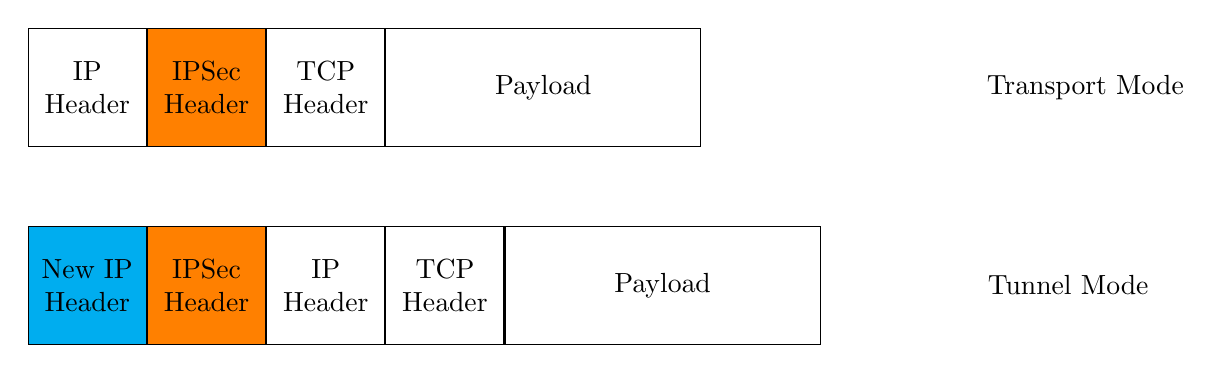
\begin{tikzpicture}[every node/.style={draw, minimum height=1.5cm, minimum width=1.5cm,align=center}]
		\node [] (iph) {IP \\ Header};
		\node [right= 0 pt of iph, fill=orange, align=center] (ipsh) {IPSec\\ Header};
		\node [right= 0pt of ipsh] (tcph) {TCP \\ Header};
		\node [minimum width=4cm, right= 0 pt of tcph] (pl) {Payload};
		\node [draw=none, right=3.5cm of pl] (lab) {Transport Mode};
		
		\node [below=1 cm of iph, fill=cyan] (niph) {New IP \\ Header};
		\node [right= 0 pt of niph, fill=orange, align=center] (ipsh1) {IPSec\\ Header};
		\node [right=0pt of ipsh1] (iph1) {IP \\ Header};
		\node [right= 0pt of iph1] (tcph1) {TCP \\ Header};
		\node [minimum width=4cm, align=center, right= 0 pt of tcph1] (pl1) {Payload};
		\node [draw=none, right=2cm of pl1] (lab1) {Tunnel Mode};
	\end{tikzpicture}

	\subsection{Authentication Header}
	L'authentication header sta tra l'header IP e quello TCP, e fornisce al destinatario informazioni per identificare la SA. L'header è strutturato come segue:

	\begin{center}
		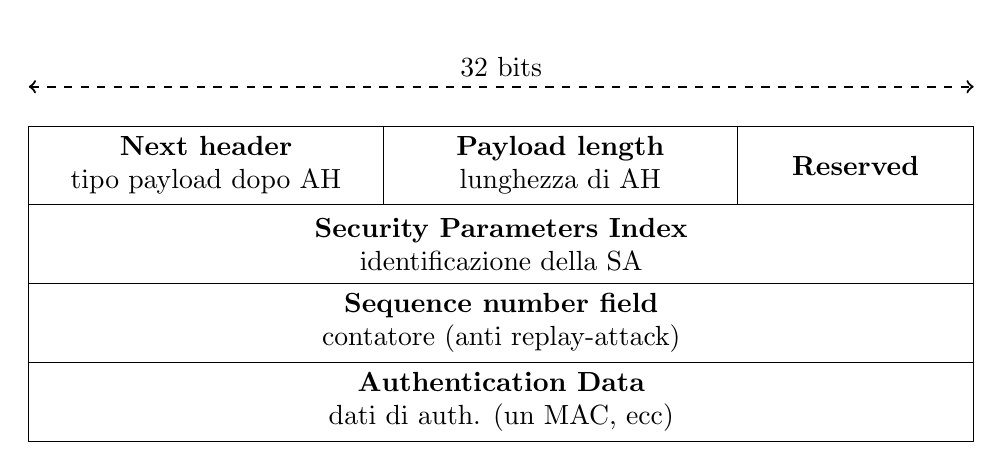
\begin{tikzpicture}[every node/.style={draw, minimum height=1cm, minimum width=12cm,align=center,node distance=-\pgflinewidth, text centered}]
			\coordinate[](A) at (-2.25,1);
			\coordinate[](B) at (9.75,1);
			\draw[<->, thick, dashed] (A) -- (B);
			\node[draw=none] at (3.75, 1.25) (lab) {32 bits};
			\node[minimum width=4.5cm] (nexth) {\textbf{Next header} \\ tipo payload dopo AH};
			\node[minimum width=4.5cm, right=of nexth] (pll) {\textbf{Payload length} \\ lunghezza di AH};
			\node[minimum width=3cm,right=of pll] (r) {\textbf{Reserved}};
			\node[](spi) at (3.75,-1) {\textbf{Security Parameters Index} \\ identificazione della SA};
			\node[](snf) at (3.75,-2) {\textbf{Sequence number field} \\ contatore (anti replay-attack)};
			\node[](adata) at (3.75,-3) {\textbf{Authentication Data} \\ dati di auth. (un MAC, ecc)};
		\end{tikzpicture}
	\end{center}
	
	L'AH in transport mode è inserito tra l'header IP e il payload, e il MAC viene fatto di tutto il pacchetto. In tunnel mode tutto il pacchetto è autenticato, il nuovo header IP, così come l'AH sono inseriti per ultimi. L'AH fornisce quindi un canale autenticato end-to-end.

	\subsection{Encapsulating Security Payload}
	L'header ESP specifica solo il protocollo di cifratura e, in maniera opzionale, per l'autenticazione.
	In transport mode (end-to-end encryption tra host che supportano IPSec) viene cifrato solo il payload del pacchetto (l'header IP rimane invariato), mentre in tunnel mode (VPN setup) tutto il pacchetto viene cifrato, ad esclusione del nuovo header IP.

	Riassumiamo i servizi offerti da IPSec come segue:\\
	\vspace{0.5cm}

	\begin{center}	
		\begin{tabular}{lccc}
			\toprule
			& \textbf{AH} & \textbf{ESP (encr. only)} & \textbf{ESP w/auth} \\
			\midrule
			Access control & \checkmark & \checkmark & \checkmark \\
			Connectionless integrity & \checkmark & & \checkmark \\
			Data origin auth. & \checkmark & & \checkmark \\
			Replayed packets rejec. & \checkmark & \checkmark & \checkmark \\
			Confidentiality & & \checkmark & \checkmark \\
			Limited traf. flow conf. & & \checkmark & \checkmark \\
			\bottomrule
		\end{tabular}
	\end{center}

	\subsection{IKE - Internet Key Exchange}
	IKE è un protocollo che, a dispetto del nome, può stabilire anche delle SA. È prodotto dall'evoluzione di vecchi protocolli come ISAKMP (framework per lo scambio di chiavi e gestione delle SA), e Oakley (joint key generation), entrambi basati su Diffie-Hellman.

	Il punto con Diffie-Hellman risiede nella PFS (\textit{Perfect Forward Secrecy}), ovvero il concetto secondo il quale un attaccante che registra un'intera conversazione cifrata non la può decifrare anche se possiede le chiavi di entrambi gli utenti. La chiave sta nel generare una chiave di sessione temporanea, non derivabile dalle informazioni salvate da ogni nodo.

	IKE procede in 2 fasi:
	\begin{enumerate}
		\item Le due entità che comunicano negoziano una SA, accordandosi sui cifrari e le funzioni di hash da usare nella fase 2;
		\item l'SA della fase 1 è usata per creare delle SA figlie, con lo scopo di cifrare e autenticare le future comunicazioni (non spiegato qua).
	\end{enumerate}

	\paragraph{Fase 1.} La fase uno può eseguire in due modalità differenti, entrambi producenti una SA: una \textbf{main mode}, molto più flessbile, con meccanismi di protezione delle identità, e  una \textbf{aggressive mode}, che scambia la metà dei messaggi, ma non prevede alcun meccanismo di protezione dell'identità. Ognuna di queste modalità ammette 4 varianti, dipendenti dal metodo di autenticazione.

	\subparagraph{Main mode.}
	La main mode è composta dei seguenti messaggi: \begin{enumerate}
		\item $I \to R: C_I, ISA_I$: l'intiator manda al responder l'SA con gli algoritmi che supporta;
		\item $R \to I: C_I, C_R, ISA_R$ il responder risponde con gli algoritmi scelti;
		\item $I\to R: C_I, C_R, X, N_I$ l'intiator manda al responder il suo $X$ di DH e un suo nonce;
		\item $I\to R: C_I, C_R, Y, N_R$ il responder risponde con il suo $Y$, calcolato da $g$ e $p$ inviati insieme ad $X$, e il suo nonce;
		\item $I\to R: C_I, C_R, \lbrace ID_I, AUTH_I\rbrace_K$;
		\item $I\to R: C_I, C_R, \lbrace ID_R, AUTH_R\rbrace_K$.
	\end{enumerate}

	I messaggi 5 e 6 sono cifrati con la chiave $K$, generata precedentemente con DH. Gli $ID$ sono identificatori di host, mentre $AUTH$ sono dati di autenticazione, dipendenti dalle varianti utilizzate.

	\subparagraph{Quick mode.} La quick mode è un condensato della main mode in 3 messaggi, senza l'autenticazione dell'identità dei due interlocutori:\begin{enumerate}
		\item $I \to R:$ autenticazione, materiale per il calcolo della chiave e proposta della SA;
		\item $R \to I:$ SA accettata, materiale di risposta della chiave;
		\item $I \to R:$ hash totale per il controllo di integrità.
	\end{enumerate}

	\section{Privacy e Anonimato}
	Cominciamo con delle definizioni a spam: \begin{itemize}
		\item \textit{Anonimity:} confidenzialità dell'identità di una persona;
		\item \textit{Privacy:} confidenzialità delle informazioni che un utente non vuole condividere.
	\end{itemize}

	Il concetto di privacy nell'IT security può essere specializzato nei concetti di \textbf{anonimity} e \textbf{data protection}.

	Ora, l'anonimato online è un concetto difficile da attuare, a causa della tipologia del traffico in internet (IP nei pacchetti, analisi del traffico, ecc) ma, esiste sicuramente un gruppo di azioni che non possono essere distinte dallo stesso traffico generato da altri utenti. Tale gruppo è detto \textbf{anonimity set}. Più grande è l'anonimity set, maggiore è lo spazio nel quale ci si può muovere rimanendo anonimi.

	Quindi, l'anonimato è tanto migliore quanti più utenti aderiscono al servizio che rende anonimi (TOR, per citarne uno).

	\subsection{Proxies}
	I proxy sono server che inoltrano il traffico in arrivo, rendendolo anonimo agli occhi dell'effettivo destinatario. Le debolezze dell'avere una struttura di questo tipo risiedono nel fatto che il proxy sa tutto dell'effettivo mittente, e il traffico rimane in ogni caso analizzabile.

	Una parziale soluzione al problema sono le proxy chain. Con un singolo proxy la situazione sarebbe la seguente: 
	
	\begin{center}
		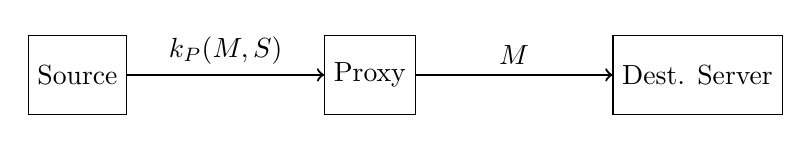
\begin{tikzpicture}[node distance= 2.5cm]
			\node [draw, minimum height=1cm](src){Source};
			\node [draw, minimum height=1cm, right=of src](proxy) {Proxy};
			\node [draw, minimum height=1cm, right=of proxy](dst){Dest. Server};
			\draw[thick,->](src)--(proxy) node[midway, above] {$k_P(M, S)$};
			\draw[thick,->](proxy)--(dst) node[midway, above] {$M$};
		\end{tikzpicture}	
	\end{center}

	dove $M$ è il messaggio e $S$ l'IP del server destinazione.
	Supponendo invece di avere una proxy chain, con cifratura a cascata, il modello diventerebbe questo: 
	
	\begin{center}
		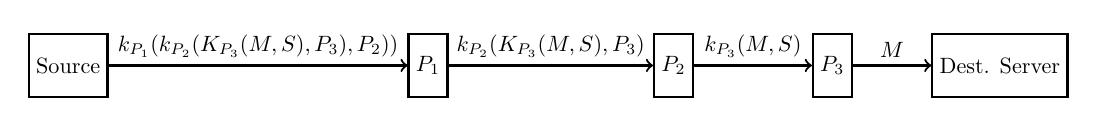
\begin{tikzpicture}[thick,scale=0.6, every node/.style={scale=0.8}]
			\node [draw, minimum height=1cm](src){Source};
			\node [draw, minimum height=1cm, right=3.8cm of src](p1) {$P_1$};
			\node [draw, minimum height=1cm, right=2.6cm of p1](p2) {$P_2$};
			\node [draw, minimum height=1cm, right=1.5cm of p2](p3) {$P_3$};
			\node [draw, minimum height=1cm, right=of p3](dst){Dest. Server};
			\draw[thick,->](src)--(p1) node[midway, above] {$k_{P_1}(k_{P_2}(K_{P_3}(M, S), P_3) , P_2))$};
			\draw[thick,->](p1)--(p2) node[midway, above] {$k_{P_2}(K_{P_3}(M, S), P_3)$};
			\draw[thick,->](p2)--(p3) node[midway, above] {$k_{P_3}(M, S)$};
			\draw[thick,->](p3)--(dst) node[midway, above] {$M$};
		\end{tikzpicture}
	\end{center}
	
	Una vistosa miglioria è data dal fatto che ogni proxy ora vede solo l'hop a lui precedente e l'hop a lui successivo. In ogni caso, l'analisi del traffico è ancora possibile. Una soluzione è data dalle \textbf{Mix networks}.

	\subsection{Mix networks}

	Sono un meccanismo costruito apposta per avere un canale anonimo, anche in presenza di un attaccante, anche supponendo che ques'ultimo conosca sorgente e destinazione e possa modificare i messaggi. 

	\paragraph{Invio di un messaggio.} Un Mix è un server che processa oggetti mail.
	In sostanza, per mandare un messaggio a B il server Mix funziona come segue: \[ \langle R_1, \langle R_0, M\rangle_{K_B}\rangle, B \rangle_{K_1} \to \langle\langle R_0, M\rangle_{K_B}, B\rangle \]

	Ogni $R_i$ è una stringa random di padding. Apparentemente sembra un normalissimo proxy, ma Mix fa anche altre operazioni per confondere l'analisi del traffico: \begin{itemize}
		\item I Mix funzionano con messaggi a lunghezza fissa (splitting di quelli lunghi, padding di quelli corti);
		\item l'ordine di arrivo dei pacchetti è mescolato, solitamente dividendo i pacchetti in gruppi differenti;
		\item l'informazione duplicata è filtrata (cross checking in tutti i gruppi);
		\item deve essere presente un certo volume di traffico $\to$ l'anonimity set è più grande $\to$ migliore l'anonimato (una possibile soluzione consiste nell'invio di pacchetti dummy da parte dei client).
	\end{itemize}

	Tavolta i mix possono generare delle "ricevute", così formate: \[ \langle C, \langle R_1, \langle R_0, M\rangle_{K_B}\rangle, B \rangle_{K_1}\rangle_{K_1^-1}  \]
	dove $C$ è una costante intera relativamente grande. Fatto ciò, il mittente può poi dimostrare di aver mandato il messaggio fornendo come prova \[ \langle\langle R_0, M\rangle_{K_B}, B\rangle \]

	Le stesse problematiche di un singolo proxy si ripresentano con un singolo mix (se è compromesso, l'anonimato scompare); in tal caso è bene scegliere un path di server Mix. Con questo meccanismo il mittente deve quindi preparare un messaggio incapsulato per ogni Mix, ossia \[R_n\langle R_{n-1}, \dots, \langle R_1, \langle R_0, M\rangle_{K_B}, B\rangle_{K_1} \dots, B_{n-2}\rangle_{K_{n-1}}, B_{n-1}\rangle_{K_n}\]

	Ogni Mix intermedio spoglia il messaggio che riceve decifrandolo e reinoltrandolo al mix successivo, fino ad arrivare al destinatario originale. 

	\paragraph{Risposta ad un messaggio.} Per rispondere ad un messaggio ricevuto da un mittente anonimo $x$, colui che risponde assembla un messaggio così formato: \[\langle\langle R_1, A_x\rangle_{K_1}, \langle R_0, M\rangle_{K_x}\rangle\] dove: \begin{itemize}
		\item $R_1$ è la stringa random (usabile anche come chiave condivisa);
		\item $K_x$ è una nuova chiave pubblica;
		\item $A_x$ è l'indirizzo di $x$.
	\end{itemize}

	Il server Mix di risposta, ricevuto il messaggio, trasforma quello che riceve in \[\langle A_x,\langle\langle R_0, M\rangle_{K_x}\rangle_{R_1}\]

	Il mittente originale del messaggio può decifrare il contenuto in quanto $K_x$ e $R_1$ sono state generate da lui quando ha mandato il primo messaggio.

	Incapsulando a cascata il sistema a mix singolo con più mix, si ottiene una situazione duale a quella per l'invio dei messaggi.

	Questo meccanismo garantisce un buon grado di anonimato, inoltre, con un buon volume di traffico, i dummy packets possono anche essere evitati. Il tracciamento del pacchetto è evitato grazie alla frammentazione/padding dei pacchetti iniziali, e sono implementati anche dei replay filter per evitare dei replay attacks.

	Ovviamente le network Mix non sono immuni di svantaggi, infatti sono ad altissima latenza (sconsigliate per il web browsing), inoltre le cifratura e decifratura sono decisamente costose, a livello computazionale.

	La difficoltà sta quindi nel creare reti anonime a bassa latenza, ad esempio usando crittografia a chiave pubblica per stabilire un "circuito" con chiavi simmetriche pairwise.

	\subsection{Randomized Routing e TOR}
	L'idea di un meccanismo del genere è quella di nascondere la sorgente del messaggio forwardando i pacchetti in maniera casuale, in tal modo i router non sanno se il mittente (= da chi ricevono il pacchetto sia effettivamente la sorgente oppure un altro router).

	Il meccanismo di routing proposto da TOR è detto \textbf{onion routing}, e suppone inizialmente che la sorgente del pacchetto stabilisca un path di router (anche compromessi) e che possa anche decidere arbitrariamente la lunghezza del path.

	Inizialmente il client stabilisce una chiave di sessione simmetrica con il primo onion router.
	Successivamente il client stabilisce una nuova chiave di sessione con il secondo router del path, con un tunnel attraverso il primo, e così via, fino alla destinazione del pacchetto. Alla fine i due client saranno collegati e potranno comunicare attraverso il path generato.

	Per mandare il messaggio alla destinazione, dal momento che Alice conosce tutte le chiavi di ogni router con cui ha stabilito la chiave di sessione, costruisce il messaggio \[ \langle \lbrace R_2, k_1\rbrace , \langle\lbrace R_3, k_2\rbrace, \dots, \langle\lbrace B, k_n\rbrace,\lbrace M\rbrace_{K_B}\rbrace_{k_n}\rangle_{k_{n-1}}, \dots,\rangle \rbrace_{k_1}\rangle \]

	Ci sono delle questioni di management della rete, quali: \begin{itemize}
		\item molte applicazioni che possono utilizzare lo stesso circuito;
		\item la necessità di mantenere dei directory servers, con liste di onion routers, le loro posizioni, le chiavi, ecc.
		\item È necessario il controllo di come i router entrano a far parte della rete (per gli attaccanti è possibile genereare dei "fake" onion router, si parla di \textbf{sybil attack}).
	\end{itemize}

	Da TOR è prevista l'esistenza di server che gestiscono gli entry point server, fornendo indirizzi e posizioni ai server di lookup, che sono consultatabili dagli utenti quando. Ovviamente tali sever devono essere accessibili da qualunque luogo,resistenti a DOS e attacchi fisici.

	L'utilizzo di questi server avviene attraverso randez-vous server, a cui l'utente si collega (tramite circuito); poi manda ad un entry point l'indirizzo (e l'autorizzazione, se necessaria) del RV server. Se l'hidden server decide di "dialogare" con l'utente, si collega al RV point.

	\subsection{Data protection e privacy policies}
	Una \textbf{privacy policy} è una specifica su come i dati degli utenti vengono utilizzati, sotto quali condizioni e quali obblighi comporti detenerli.

	Le policies più comuni descrivono: \begin{itemize}
		\item Controllo sull'accesso ai dati;
		\item Azioni richieste prima di accedere ai dati;
		\item Azioni che devono essere fatte entro un certo periodo di tempo (informare il data owner ogni volta che i suoi dati sono utilizzati);
		\item Restrizioni sulla distribuzione dei dati;
		\item Restrizioni sui motivi per i quali i dati sono utlilzzati;
		\item Restrizioni sul mantenimento dei dati;
		\item Meccanismi di protezione obbligatoria dei dati (e.g. backup cifrati);
		\item Dovere di mantenre i dati aggiornati.
	\end{itemize}

	La formalizzazione delle politiche sulla privacy avviene attraverso linguaggi machine-friendly (P3P, W3C), che possono eventualmente essere portati in formati computer-readable (XML).
	Altri privacy oriented languages sono SAML, EPAL (da IBM), SOAP (Microsoft metadata).

	Esistono poi dei meccanismi di rinforzo delle politche sulla privacy quali la \textit{Online Privacy Alliance}, un gruppo si 50 compagnie che adottano un unico insieme di linee guida per la preservazione e l'utilizzo dei dati, il tutto controllato e monitorato da terze parti.

	\section{Intrusion Detection}
	\subsection{Intruder}
	Prima di parlare di intrusioni in sè, distringuiamo i vari e possibili tipi di intrusi: \begin{itemize}
		\item \textbf{Masquerader}: un individuo non autorizzato all'uso del pc;
		\item \textbf{Misfeasor}: un utente legittimo che accede non autorizzato alle risorse;
	\end{itemize}

	Al di là dei singoli utenti intrusi, si può parlare anche di gruppi di hacker organizzati, anche sotto controllo governativo, più proni all'uso di backdoor o RAT per tornare al bersaglio quando sia necessario.
	
	\subsection{Detection delle intrusioni}
	I meccanismi di intrusion detection mirano a identificare e se necessario bloccare tali tentativi (ovviamente non sono infallibili), ma in ogni caso agiscono da deterrente e raccolgono informazioni utili per migliorare la sicurezza del sistema in sè. L'unico problema è che gli IDS assumono che l'intruso si comporti in maniera differente da un utente normale, inoltre tendono ad avere un fail ratio relativamente alto, dovuto all'alto numero di falsi positivi/negativi che tendono ad avere.

	Ci sono molteplici approcci all'intrusion detection, ossia: \begin{itemize}
		\item \textbf{Rilevamento statistico delle anomalie}: sono un insieme di meccanismi basati su threshold (azioni ripetute, inusuali per un utente standard), oppure anche meccanismi profile-based, che mirano a costruire un profilo per ogni utente e usarlo per rilevare possibili anomalie nei comportamenti. 
		\item \textbf{Rilevamento basato su regole}: meccanismi orientati verso la rilevazione di azioni che esulano dai comportamenti standard, oppure che riconoscono tentativi di violazione al sistema basati su una conoscenza pregressa delle azioni malevole;
	\end{itemize}

	\paragraph{Audit records.} Sono dei record studiati per raccogliere ogni attività utente svolta.
	Ci sono due approcci comuni: \begin{itemize}
		\item \textbf{Audit record nativi}: sono posizionati su ogni workstation;
		\item \textbf{Audit record detection-specific}: sono generati da una facility dedicata.
	\end{itemize}

	Ogni audit record è strutturato con i seguenti campi:\begin{enumerate}
		\item Soggetto;
		\item Azione svolta;
		\item Oggetti su cui l'azione si è svolta;
		\item Eccezioni varie, se presenti;
		\item Risorse utilizzate;
		\item Timestamp.
	\end{enumerate}

	

	\paragraph{IDS distribuiti.} In reti molto ampie, l'idea migliore è quella di usare IDS distribuiti, per coordinare la difesa dell'intera rete. Ciò pone alcuni problemi, quali: \begin{itemize}
		\item formati di audit record differenti;
		\item integrità e confidenzialità dei dati in rete;
		\item architettura (centralizzata vs decentralizzata).
	\end{itemize}

	Il modello più classico di IDS di rete è costituito da 3 entità:\begin{itemize}
		\item \textbf{Host agent module}: uno per ogni host, raccolgono dati lavorando in background sul sistema monitorizzato;
		\item \textbf{LAN monitor agent module}: opera analogamente al'host agent module, ma lavora sul traffico di rete;
		\item \textbf{Central manager module}: modulo che raccoglie i dati dagli altri due, li processa e mette insieme i report ricevuti per verificare possibili intrusioni.
	\end{itemize}
	Questo schema è disegnato per essere indipendente dal sistema operativo host.

	Ogni agente procede quindi filtrando l'informazione di interesse, formattando l'output generando un \textit{Host Audit Record} (HAR), che viene passato ad un modulo di analisi per controllare se nel record generato vi sono attività sospette. In caso sia rilevata un attività sospetta, i dati vengono inviati al central manager che, in alternativa, può anche eseguire una query all'agente per ottenere dati che sono necessari alla correlazione con i dati ricevuti da altri agenti.

	\subsection{Honeypots}
	Gli honeypots sono sistemi esca per ingannare gli attaccanti e indurli a credere di stare attaccando un sistema chiave. Spesso sono correlati di finti dati sensibili per renderli maggiormente credibili. 

	Gli honeypot fornisono una serie di vantaggi, in quando consentono di:\begin{itemize}
		\item raccogliere dati relativi all'attaccante (quando sono dotati di sistemi di monitoraggio);
		\item mettono al riparo i veri sistemi sensibili;
	\end{itemize}

	Gli honeypot sono sostanzialmente delle macchine volutamente vulnerabili, e sono posizionabili in diversi postazioni nella rete: \begin{itemize}
		\item esternamente al firewall di rete $\rightarrow$ tracciano attacchi ad indirizzi IP non usati all'interno della rete, non comportano rischi per i sistemi vitali. Tuttavia, non hanno possibilità di ingannare gli attaccanti interni.
		\item nella DMZ $\rightarrow$ l'amministratore di rete deve assicurarsi che gli altri sistemi della DMZ siano adeguatamente protetti, inoltre il firewall di solito blocca richieste provenitenti dalla DMZ.
		\item completamente interno alla rete $\rightarrow$ cattura gli insider, permette di individuare errori nella configurazione del firewall. Di contro, se l'honeypot è compromesso, tutta la rete è vulnerabile, in più il firewall deve essere configurato in modo da permettere il traffico da e verso l'honeypot, il che espone la rete ai potenziali rischi di cui sopra.
	\end{itemize}

	\subsection{Gestione delle password}
	Le password andrebbero salvate in forma cifrata (UNIX usa DES con sale), magari con funzioni hash crittografiche. Tuttavia è necessario proteggere anche il file dove la password sono salvate.

	Studi recenti e antichi dimostrano che il problema maggiore della password sono gli utenti, perchè le scelgono troppo semplici o corte. In tal senso è importante imporre linee guida per la creazione della password (lunghezza minima, variazione dei caratteri, evitare parole di uso comune), ma ancora meglio sarebbe se i computer generassero le password che servono.

	L'approccio migliore in ogni caso è il controllo proattivo, ossia lasciare che l'utente scelga la password e lasciare che sia il sistema a decidere se accettarla oppure no.

\end{document}